%%%%%%%%%%%%%%%%%%%%%%%
%%% DOCUMENT SETTINGS
%%%%%%%%%%%%%%%%%%%%%%%
\documentclass[11.0pt]{exam}
\printanswers % Uncomment to show answers
\include{formatAndDefs}
%%%%%%%%%%%%%%
%%% PACKAGES
%%%%%%%%%%%%%%
\usepackage{amsmath,amsfonts,amssymb,amsthm} % math fonts and symbols
\usepackage{bbm} % Math blackboard font
\usepackage{enumitem} % For reference enumerations lists
\usepackage{textcomp} % some symbols (like copyright)
\usepackage[top = 2cm, bottom = 2cm, right = 1.2cm, left = 1.2cm, paper = a4paper, headheight = 6cm]{geometry} % Margins setup
\usepackage{xcolor} % Colors
\usepackage{pgfplots}
\usepackage{spalign}
%%%%%%%%%%%%%%%%%%%%%%%%%%
%%% MACROS AND COMMANDS
%%%%%%%%%%%%%%%%%%%%%%%%%%
\definecolor{CUNEForange}{RGB}{237, 114, 1}
\newcommand{\N}{\mathbb{N}} % natural number set
\newcommand{\R}{\mathbb{R}} % real number set
%%%%%%%%%%%%%%%%%%%%%%%%%%%%%%%%%
%%% HEADER AND FOOT 
%%%%%%%%%%%%%%%%%%%%%%%%%%%%%%%%%
% Defining information
\newcommand{\degree}[1]{Bachelor in Philosophy, Politics and Economics}
\newcommand{\shortdeg}[1]{PPE}
\newcommand{\exam}[1]{2nd Midterm}
\newcommand{\subject}[1]{Mathematics}
\newcommand{\theyear}[1]{2023/24}
%\newcommand{\ccauthor}[1]{A. Azze \textcopyright\the\year}
\newcommand{\thedate}[1]{12 1 2023}
\newcommand{\university}[1]{CUNEF University}
% Setting header
\usepackage{fancyhdr}
\pagestyle{fancy}
\renewcommand{\headrulewidth}{0.1mm}
\renewcommand{\footrulewidth}{0.1mm}
% \renewcommand{\sectionmark}[1] % To avoid sections' titles being displayed on the header
{\markright{\MakeUppercase{}}}
\setlength\headsep{0.5cm}
% Header and footer
\fancyhead[L]{\degree{} \\ \subject{} - \theyear{}}
\fancyhead[R]{\thedate{} \\ \ccauthor{}}
\fancyfoot[L]{\university{}}
\fancyfoot[C]{}
\fancyfoot[R]{\thepage}

%%%%%%%%%%%%%%%%%%%%%%%%%
%%% DOCUMENT CONTENT
%%%%%%%%%%%%%%%%%%%%%%%%%
\begin{document}
%--- Instructions ---%
\begin{center}

    {\Huge \textbf{\exam{}}}
    \vspace{0.7cm}

    \begin{flushright}
        \textbf{Time Limit:} 50 minutes
    \end{flushright}
    \vspace{-0.2cm}
    
    \fbox{\parbox{\textwidth}{\centering 
        \begin{enumerate}[leftmargin = 0.5cm, label = $\bullet$, rightmargin = 0.2cm]
    
            \item \textbf{Every non-trivial calculation and claim in the exam must be properly justified.}

            \item The use of calculators is not necessary and therefore not allowed.

            \item Digital devices such as mobile phones, tablets, and laptops, as well as internet access, are forbidden.

            \item You can use physical resources such as books, notes, and other printed materials to assist you during the exam.
 
        \end{enumerate}
    }}
\end{center}
%--- Instructions ---%

%--- Questions ---%

\begin{questions}

% Question
\question[3]
    A square matrix $A$ is called idempotent if $A^2 = A$.
    \begin{enumerate}[leftmargin = 0.5cm, label = (\alph*), rightmargin = 0.2cm]
        \item Check if the matrix 
        $\begin{pmatrix}
        2  & -2 & -4 \\
        -1 & 3  & 4 \\
        1  & -2 & 3
        \end{pmatrix}$ is idempotent.
        \item Show that, if $AB = A$ and $BA = B$, then $A$ and $B$ are both idempotent.
        \item Show that if $A$ is idempotent, then $A^n = A$ for all positive integers $n$.
    \end{enumerate}
% Solution
%\begin{solution}[0cm]
%    \begin{enumerate}[leftmargin = 0.5cm, label = (\alph*), rightmargin = 0.2cm]
%\end{solution}

% Question
\question[3] Consider the following plot, representing the demand a supply sets in a market.
\[D=\{p+q=5\},\qquad S=\{p-q=1\}.\]

\begin{center}
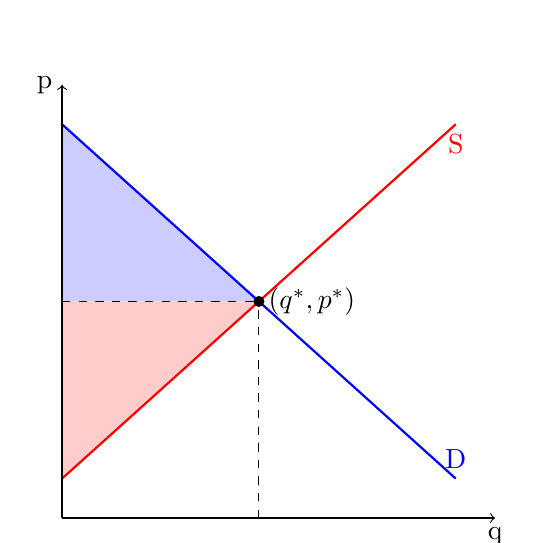
\begin{tikzpicture}
	% Área de excedente del consumidor (azul)
	\fill[blue!20, domain=0:2.5, variable=\x]
	(0,5) to (2.5,2.75) -- (0,2.75) -- cycle;
	% Área de excedente del productor (rojo)
	\fill[red!20, domain=2.5:4.5, variable=\x]
	(0,0.5) to (0,2.75) -- (2.5,2.75) -- cycle;
    % Curva de demanda
    \draw[thick, blue] (0,5) to (5,0.5) node[above] {D};  
    % Curva de oferta
    \draw[thick, red] (0,0.5) to (5,5) node[below] {S};
    % Eje de las cantidades
    \draw[->] (0,0) -- (5.5,0) node[below] {q};
    % Eje de los precios
    \draw[->] (0,0) -- (0,5.5) node[left] {p};
    % Punto de equilibrio
    \coordinate (equilibrium) at (2.5,2.75);
    \fill[black] (equilibrium) circle (2pt) node[right] {$(q^*,p^*)$};
    % Línea horizontal punteada en el punto de equilibrio
    \draw[dashed] (0,2.75) -- (2.5,2.75);
    \draw[dashed] (2.5,0) -- (2.5,2.75);
\end{tikzpicture}
\end{center}

    In this figure, $(q^*,p^*)=(2,3)$ represents the equilibrium point. Recall that the \emph{consumer surplus}, shown in blue, is computed as the area under the graph of $p_d(q)$ between $0$ and $q^*$ minus the area of the rectangle of side $p^*q^*$, that is, \[\int_0^{q^*}p_D(q) dq-p^*q^*.\] Write the formula to compute the \emph{productor surplus}, shown in red, and compute its value in this example.
%% Solution
%\begin{solution}[0cm]

%\end{solution}

% Question
\question[2]
Determine if the following integral converges and draw the area it represents.
\[\int_1^{\infty} 3x^{-\frac{5}{3}} dx\]
% Question
\question[2] Write the following system of linear equations in matrix form, and solve it using the inverse matrix of the coefficient matrix.
\[
  \spalignsys{
    x+2y-z=5 ;
    y+z=-1 ;
   -x+z=2
  }
\]
What would be the answer if the determinant of the coefficient matrix is 0?    

% % Question
% \question[2]
% The tobacco market is a monopoly, with supply and demand sets
% \begin{align*}
%     S = \{(q, p) : 15p − 2q = 20\},\quad D = \{(q, p) : q + 5p = 40\}.
% \end{align*}
% Given that the government has imposed an excise tax of $T$ dollars to the tabaco market:

% \begin{enumerate}[leftmargin = 0.5cm, label = (\alph*), rightmargin = 0.2cm]
        
%     \item Define the governments revenue function in terms of the excise tax and the number of units sold.

%     \item Find the excise tax that maximizes the government revenue.
        
% \end{enumerate}
% % Solution
% \begin{solution}[0cm]
%     Solution
% \end{solution}

% % Question
% \question[2]
%     A firm manufactures two goods, $X$ and $Y$. The market price of these goods is unaffected by the level of the firm's production. The firm's cost function is $C(x, y) = 2x^2+ xy + 2y^2$. The market prices for $X$ and $Y$ are $12$ and $18$ dollars per unit, respectively. Determine the number of units of each good that the firm should produce to maximize its profit.  
% % Solution
% \begin{solution}[0cm]
%     Solution
% \end{solution}

% % Question
% \question[2]
%     A wine dealer has certain amount of units of barrels of wine, which he can sell today at $K$ dollars or wait for a better deal. The price of his barrels of wine increases in time according the the function $Kt^n$, for $n \in \N$. Assume that the market holds an interest rate of $r \R_+$ on continuously compounding levels, that is, $x$ today's dollars equal $xe^{-r t}$ dollars $t$ units of time ahead.
    
%     \begin{enumerate}[leftmargin = 0.5cm, label = (\alph*), rightmargin = 0.2cm]

%         \item Define the profit made by selling the barrels of wine at time $t$.
    
%         \item When should the dealer sell the barrels of wine to maximize his profit? Hint: you can use Problem 3 to ease the optimization.
    
%     \end{enumerate}
% % Solution
% \begin{solution}[0cm]
%     Solution
% \end{solution}

% Question


\end{questions}	

\end{document}